The rate at which climate changes today is mostly due to the concentration
of anthropogenic \gls{GHG} in the atmosphere \cite{IPCC_CO2_budget}. Therefore, the \gls{GHG} emissions from human activities must be mitigated to prevent further environmental damage. Energy consumption, mainly from fossil fuels, is the main contributor: it is responsible for 75\% of \gls{GHG} emissions, the remaining 25\% originating from agriculture and industrial processes \cite{ourworldindata_CO2_world}. The Kaya identity is an economic formulation stating that the total emission level of the \gls{GHG} can be expressed as the product of four factors: human population, \gls{GDP} per capita, energy intensity (per unit of GDP), and carbon intensity (emissions per unit of energy consumed) \cite{kaya1997environment}. From an energy point of view, this identity can be adapted by replacing the economic metric, \gls{GDP}, by the \gls{EUD}, see Equation (\ref{eq:equality_GHG}). \gls{EUD} is the energy service required by the final consumer. In Equation (\ref{eq:equality_GHG}), the first factor on the right-hand side represents the \gls{GWP} of the primary energy mix, the second is the inverse of the efficiency and the third is the energy intensity per capita.

\begin{equation}
\label{eq:equality_GHG}
\mathrm{GHG} =  \frac{\mathrm{GHG}}{\text{Primary energy}} \times \frac{\text{Primary energy}}{\mathrm{EUD}}\times \frac{\mathrm{EUD}}{\text{Population}} \times \text{Population}\\
 \end{equation}

Such an identity is criticized for the arbitrary choice of variables, the non-independence of them usually leading to the rebound effect and its encompassing approach that does not appropriately mirror the heterogeneity of the situation \cite{IPCC2000}. Considering the expected growing trend of the Population, Equation (\ref{eq:equality_GHG}) highlights three levers of action that should be activated to reduce \gls{GHG} emissions and favour the energy transition \cite{dodson2020population,scovronick2017impact}: renewables, efficiency and sufficiency. 

Focusing on the levers that are within the grasp of engineering studies, this thesis addresses the two ``technical'' levers of the energy transition identified in Equation (\ref{eq:equality_GHG}): renewables and efficiency. This focus is aligned with the current European policies binding the Member States of the European Union. For instance, the Renewable Energy Directive (RED) III, published in October 2023 \cite{REDIII}, states that ``the Union’s climate neutrality objective (by 2050) requires a just energy transition which leaves no territory or citizen behind, an increase in energy efficiency and significantly higher shares of energy from renewable sources in an integrated energy system''.% (\ie 42.5\% of the Union's gross final consumption of energy by 2030). 

Despite the growing echo it finds in the scientific community \cite{o2018good}, sufficiency is lacking in the RED III. Explicitly mentioned by the IPCC for the first time in 2022 \cite{IPCC2022}, it is defined as ``\emph{a strategy for reducing, in absolute terms, the consumption and production of end-use products and services through changes in social practices in order to comply with environmental sustainability while ensuring adequate social foundation for all people}'' \cite{lage2023citizens}. Due to its intrinsically political nature, studying sufficiency requires an interdisciplinary approach involving economy, sociology, psychology and political science, and is beyond the scope and knowledge of engineering research \cite{schmidt2015interdisciplinary}. Among all the lenses through which it is necessary to assess sufficiency policies, one of the objectives of this work is to support these interdisciplinary projects by providing informed techno-economic guidelines.\\

\noindent
To ensure the energy supply of a growing and more demanding population in the context of an environmental crisis, major transformations are needed (see Figure \ref{fig:intro:IEA_WEO_2019}). Similarly to the RED III, the transformations identified by the \citet{iea2020world} focus on technical aspects, disregarding the sufficiency.  The technical transformations that can be brought to the energy system concern both the primary energy sources and the technologies used to convert more efficiently these resources into the \gls{EUD} \cite{iea2020world,luderer2018residual}. 

\begin{figure}[ht!]
\centering
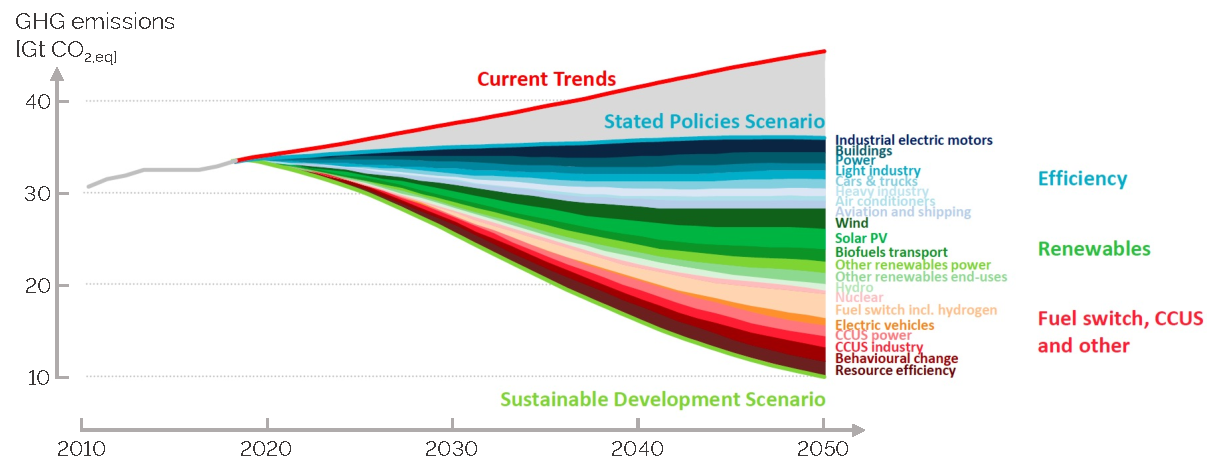
\includegraphics[width=\textwidth]{IEA_WEO_2019.pdf}
\caption{Energy-related \ce{CO2} emissions and reductions by sources in the Sustainable Development Scenario of the \citet{iea2020world}.}
\label{fig:intro:IEA_WEO_2019}
\end{figure}

Changing primary energy sources corresponds to integrating more renewables. \gls{VRES} like wind and solar are the keystones to defossilise the energy system but they face challenges related to their intermittency and space disparity.  With a growing share of \gls{VRES}, sector coupling and electrification, with electrical heat pumps or Battery Electric Vehicles (BEV), are essential to absorb the surplus of electricity from these intermittent production means \cite{robinius2017linking} and integrate them cost-effectively \cite{brown2018response, limpensECOS2021}. 

However, direct electrification is not foreseen to be cost-competitive for some sectors such as marine, aviation and heavy-duty transport \cite{horvath2018techno, brynolf2018,IEA2021}. Moreover, transport and long-term storage of renewable electricity are not optimal with electricity-based solutions, \eg {DC} lines or batteries. This is why, to reach the objective of sustainable development, after increasing the efficiency of the system, more renewables is associated with a ``fuel switch'' (see Figure \ref{fig:intro:IEA_WEO_2019}). 

The fuel switch consists in replacing fossil fuels with new energy carriers.  Among them, \textit{electrofuels} are promising solutions to tackle the challenges related to renewable electricity \cite{rozzi2020}. These fuels represent energy carriers where electricity has the major share in the energy balance of the fuel. In practice, this electricity is mainly converted into hydrogen through electrolysis and then potentially upgraded into more complex fuels such as methane, methanol or ammonia. 

Electrofuels offer three main advantages: infrastructure compatibility, capacity to link sectors (\ie from electricity to mobility, heat, or industry) and storage. Given their similar physicochemical properties, electrofuels could substitute fossil in technologies that are already in place today. An example is ammonia-hydrogen blends burned in spark ignition engines \cite{lhuillier2020experimental} or \gls{CHP} applications \cite{pochet202022}.

Electrofuels can also couple energy and non-energy sectors \cite{Stancin2020}. For instance, electricity from \gls{VRES} can be converted into ammonia through the Haber-Bosch process and subsequently transformed into fertiliser, coupling the power and agro-industrial sectors \cite{verleysen2020can}. 

Concerning storage,  batteries exhibit limited storage capacity (up to 10\,MWh) and self-discharge losses. On the contrary, electrofuels are promising solutions for high capacity (from 100 GWh) and long-term storage of energy \cite{child2018role, dias2020energy} (Figure \ref{fig:intro:Storage_electrofuels}). In their analysis of the German transport sector in 2050, \citet{millinger2021electrofuels} highlighted that producing electrofuels can represent an efficient usage of the ambient \ce{CO2} to supply hydrocarbon fuels while limiting the curtailment of \gls{VRES}. Moreover, gas networks present much more storage potential than electrical networks: 50 times more in Germany and 300 times more in France \cite{Rosa2017}. 

\begin{figure}[htbp!]
\centering
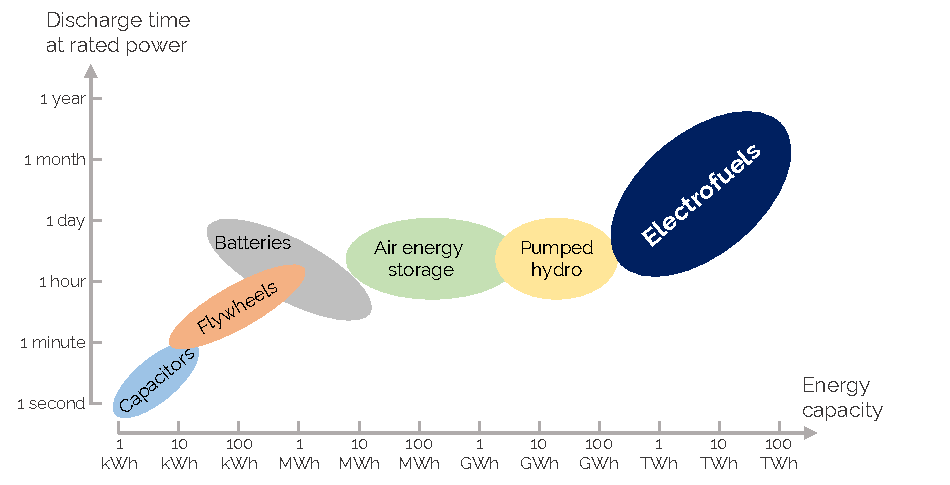
\includegraphics[width=0.9\textwidth]{Storage_electrofuels.pdf}
\caption{Energy carriers and technologies to store electricity. Electrofuels provide a solution for high-capacity and long-term storage of energy. Graph adapted from \cite{ISPT2017}.}
\label{fig:intro:Storage_electrofuels}
\end{figure}

\newpage
Even if the share of electricity will increase in the energy system through the electrification of the end-use demand, gaseous and liquid fuels will keep on being big players during, and after, the energy transition \cite{Ahlgren2012}. In other words, hydrocarbons, currently produced from fossil resources, will still be composed of carbon in a renewable world. This is why this thesis rather uses ``defossilisation'' rather than ``decarbonisation'' as carbon will still play a key role in the energy transition that aims at carbon neutrality where there is no additional, if no removal, of \gls{GHG} emissions in the atmosphere \cite{mertens2020carbon}. 

Besides electrofuels, ``\emph{biofuels}'', ``\emph{synthetic fuels}'', ``\emph{renewable fuels}'' or even ``\emph{sustainable fuels}'' will play a key role in the transition. To avoid the confusion between all these ``alternative'' fuels and thereby reduce misunderstanding in political or academic discussions, we have developed a comprehensive and harmonised taxonomy (see Appendix \ref{app:Taxonomy}).  In the rest of this thesis, the electro --- and bio --- fuels, imported from the exterior of the considered energy system, are regarded as renewable with no associated \gls{GWP}. 

To harvest the maximum potential of synthetic fuels in a sustainable transition and maximise the overall system efficiency \cite{mathiesen2015}, it is necessary to study the integration of these fuels within a whole-energy system which is multi-sector and accounts for multiple energy carriers \cite{contino2020whole}. To reach this goal, an energy system optimisation model (ESOM) can optimise the design and the operation of the system to minimise, for instance, its costs or its emissions \cite{zeng2011review}. 

In the field of energy system planning and scenario analysis, \citet{yue2018review} highlighted that most ESOMs use a deterministic approach (75\% of the 134 reviewed studies). However, the models and their numerous composing parameters are inherently uncertain especially when it comes to defining an energy transition strategy for a large-scale system such as a country. Given the lifetime of energy conversion technologies, such a strategy implies decisions with long-term impacts (20 to 50 years) where forecasts can be highly unreliable \cite{Moret2017}. This long-term and large-system optimisation motivates the need to account for \gls{UQ}, which is considered a major challenge of such models in the literature \cite{pfenninger2014energy}. %This challenge, along with a large number of uncertain parameters (more than a hundred), leads to the "curse of dimensionality" \cite{kuo2005lifting}, where the computational burden rapidly explodes with the number of considered uncertain parameters.

On top of dealing with these uncertainties, the reality of decision-makers leads to a limited foresight into the future \cite{poncelet2016myopic}. In a perfect foresight approach, decision-makers would be able to, from now on, see the ``finish-line of the transition'' in 2050 and accordingly make the planning decisions once and for all. On the contrary, they uncover the realisation of these uncertainties step-by-step, in a ``myopic'' way, and progressively act on them to, hopefully, meet the set target to reduce the anthropogenic \gls{GHG}. In the objective to respect an overall \ce{CO2} budget rather than to follow a prescribed \ce{CO2}-emissions trajectory, there is a need for a framework to explore these multiple transition pathways and provide insight into intermediate milestones not to miss. On top of the ``what to do?'', this framework should aim at helping the policymakers to answer the  question ``how to do it?''.

The robustness of transition pathways provided by ESOMs is an essential question due to their sensitivity to uncertain factors. A variety of techniques are used to assess this robustness including Monte-Carlo analysis, stochastic programming or robust optimisation \cite{yue2018review}. However, the robustness is commonly assessed to evaluate the sensitivity of the total cost (objective function) to input parameters.  Given the complexity of whole-energy system models, the time scale of the transition and the large number of uncertainties, only considering the total cost does not give information on the sensitivity of the design strategy, \ie the investment decisions. For instance, total cost might consist of excessive upfront investments and a better balance of \gls{CAPEX} and \gls{OPEX} might be preferable despite a slightly higher total cost. \citet{moret2020overcapacity} proposed a method to assess the robustness of a design by investigating the potential overcapacity needed to face uncertainties. However, their work focused on the power sector only and on the target future year of 2035.  Instead, an objective of this thesis is to tackle these two challenges: go beyond the total transition cost and provide more details on the sensitivity of the design to uncertainties while assessing a whole-energy system over its whole transition.\\

\noindent
``\textit{Our task is not to foresee the future, but to enable it}''\footnote{Saint-Exupéry in Citadelle, 1948}. Rather than trying to answer the question ``What could happen in the future?'', this work addresses the ``What could or should we do to make the future possible?''. This thesis aims at providing decision-makers with information and new methods considering the intrinsic uncertainties of the future.  In that spirit, the research questions are described as follows:
\begin{itemize}
\item What can be the role of electrofuels in the transition pathways of a whole-energy system considering uncertainties,  limited foresight, and a given \ce{CO2} budget? What are the key uncertainties driving their local production or import?
\item How to explore the multiple possible pathways through the optimisation of a sequence of actions to support an energy transition?
\item How to assess the robustness of a transition roadmap whilst developing strategy and designing possible pathways?
\end{itemize}

To answer these questions, several tasks have been carried out on the whole-energy system model accounting for the uncertainties, the method to explore the myopic pathway of such a system and the approach to assess the robustness of a pathway roadmap. 

The model developed and used in the context of this thesis is EnergyScope Pathway \cite{limpens2024pathway}. First introduced by Limpens in his PhD thesis \cite{limpens2021generating}, this model optimises the design and the operation of a whole-energy system over several decades and accounts for transition pathways from an existing system to a long-term target, \ie 2050. Based on this model originally implemented for a perfect foresight approach, we have developed the myopic method in which the whole time horizon (30 years) is optimised through a sequence of 10-year time windows with 5-year overlaps.

To address the question of the role of electrofuels, they have been integrated into the pre-existing model, focusing on four molecules: hydrogen, methane, ammonia and methanol. Moreover, given their current and (expected) future role in the sector of the \gls{NED}, we have added this sector to the model with a similar level of detail as for the other sectors of the system, \ie electricity, heat and transport. 

To account for uncertainties, uncertainty characterisation and quantification have been applied by adapting the works of \citet{Moret2017PhDThesis} and \citet{coppittersthesis}, respectively. In his thesis, \citet{Moret2017PhDThesis} developed a framework to obtain uncertainty ranges for a variety of parameters such as cost of purchasing and availability of resources or investment cost and efficiency of technologies. These ranges have then been sampled and propagated through the EnegyScope Pathway via the RHEIA framework developed by \citet{coppittersthesis}. Using the surrogate modeling approach called \gls{PCE}, this framework allows identifying the uncertain parameters with the biggest impact on the variation of total transition cost or other outputs of interest such as the imported amount of electrofuels. 

To explore the different pathway trajectories in this myopic optimisation process, we have applied the \acrfull{RL} method. In this branch of machine learning, an ``agent'' is trained through its interactions with its environment, EnergyScope Pathway, to optimise its policy, \ie the sequence of actions to take to support the transition. 

Finally, in the objective to assess the sensitivity to uncertainties of different transition roadmaps, we have defined an approach to come up with a ``robustness metric''. This approach is based on \gls{PCA} where directions capturing the widest design variations are identified and serve as a reference frame. Roadmaps resulting from perfect foresight optimisation have been tested in myopic and uncertain pathways. The results of these myopic runs have then been ``projected'' on the aforementioned frame to be able to compare the robustness of different roadmaps with each other.

All this work has been applied to the case of Belgium, a densely populated country with a limited potential of renewable energies, which represents roughly half of the forecast energy demand \cite{Limpens2020}. This makes it a challenging case to go from a highly fossil-dominated system in 2020 (73\% of the primary energy mix \cite{spf_economy_2022}) to carbon neutrality by 2050.\\

\noindent
This thesis is composed of five chapters to provide answers to the different research questions (see Figure \ref{fig:intro:Thesis_Structure}). Chapter \ref{chap:chap_methodo} details the tools and methods we used. It starts with the main constraints, parameters and variables of EnergyScope Pathway, the whole-energy system optimisation model. Then, it explains the \acrfull{UQ} approach and the way it has been adapted to the case of Belgium and its transition pathway. Finally, general fundamentals and more case-specific considerations are brought up about the \gls{RL} and \gls{PCA}-based robustness approaches.

Chapter \ref{chap:case_study} presents the case study of this work: Belgium and its energy transition. Without exhaustively detailing the data used from the work of \citet{limpens2021generating}, this chapter focuses on the main contributions of this work regarding the case study: the \gls{NED}, the implementation of electrofuels and their respective routes of production and consumption, limiting  the cumulative emissions of the transition to a certain \ce{CO2} budget rather than a prescribed emissions-trajectory and the data related to \gls{SMR} as an option to produce nuclear-based electricity in the future.

Chapter \ref{chap:atom_mol} details the results of the \gls{GSA} carried out on the Belgian energy transition under uncertainties. On top of the impact of uncertainties on the total transition cost and the system design in general, we analyse the impact of having new nuclear (``atom'') capacities by 2040 onward and the driving parameters on the import of electrofuels (``molecules''): the so-called atom-molecules dilemma.

In Chapter \ref{chap:chap_RL}, we detail the rules of the ``\gls{RL} game''. In other words, we define the action and state spaces as well as the reward function driving the agent's behaviour in its quest to optimise its policy. Then, we analyse the results of the agent's learning process and compare these results with the perfect foresight approach.  Chapter \ref{chap:chap_RL} focuses on the robustness of a policy as its ability to maximise the chances to succeed a myopic transition under uncertainties to meet a \ce{CO2} budget.

Chapter \ref{chap:chap_RobPol} assesses the robustness of different technological roadmaps as their ability to limit the investment into additional capacities when tested in myopic conditions. Three roadmaps resulting from different deterministic perfect foresight optimisation, are presented: REF, SMR and ROB. The first one, the reference case, considers nominal values for all the uncertain parameters. The SMR case is the one introduced in Chapter \ref{chap:atom_mol} where we allow the model to install \gls{SMR} from 2040 onward. Eventually, the ROB case accounts for the highest values of uncertain parameters having the biggest impact on the total cost of transition (\ie cost of purchasing fossil fuels and renewable electrofuels, industrial \gls{EUD}, discount rate and variable \gls{OPEX} of technologies).

Finally, we draw the main conclusions from this work: near-term actions are needed to respect the ambitious \ce{CO2} budget and investing in electrofuels provides robustness to uncertainties and limited foresight into the future.  Perspectives are suggested for future research on further developments and uses of the methodological tools.


\begin{figure}[htbp!]
\centering
\includegraphics[width=\textwidth]{Thesis_Structure.pdf}
\caption{Structure of the thesis. Beyond Chapter 2 that describes the case study of Belgium, Chapters 3, 4 and 5 collect the analyses resulting from the application of the different methodologies developed in Chapter 1. Given the (quasi-)independence of the analyses presented in the last three chapters, they can be read separately.}
\label{fig:intro:Thesis_Structure}
\end{figure}